% Chapter Template

\chapter{Analysis of Feed Forward Derating Control Scheme With SOWFA.} % Main chapter title

\label{Chapter6} % Change X to a consecutive number; for referencing this chapter elsewhere, use \ref{ChapterX}

\lhead{Chapter 6. \emph{Analysis of Feed Forward Derating Control Scheme With SOWFA.}} % Change X to a consecutive number; this is for the header on each page - perhaps a shortened title

%----------------------------------------------------------------------------------------
%	SECTION 1
%----------------------------------------------------------------------------------------

\section{Introduction} \label{section6-1}

Chapter \ref{Chapter4} investigated the benefits and feasibility of derating a downwind turbine based on a feed forward signal from an upwind turbine. The feed forward derating control scheme developed in chapter 4 monitors the rotor speed of the upwind turbine for large rotor overspeeds, which are indicative of large wind gusts. When those large rotor overspeeds are detected, the downwind turbine is smoothly transitioned to derated operation until the gust passes. Derating a turbine reduces power generation, but also decreases both structural loads and rotor speed, making that turbine less sensitive to the detrimental effects of a large wind gust. By derating the downwind turbine only when the upwind turbine detects a large wind gust, the downwind turbine gains the benefits of derating (reduced loads and overspeeds) when they are needed most while keeping the cost of derating (reduced energy generation) in check.

The control scheme was evaluated using a series of FAST simulations, which showed promising results (Section \ref{section4-6}). The control scheme reduced peak structural loads and damage equivalent loads (DEL) while decreasing rotor overspeeds enough to avoid emergency shutdowns of the downwind turbine. The control scheme did reduce electricity generation, but the reduction was small and would likely be much less than the power lost in an emergency turbine shutdown. Though these results are promising, the simulation methodology used to generate them has several noteworthy limitations. First, these simulations did not model emergency turbine shutdowns due to rotor overspeeds. Second, to simulate this system in FAST we had to assume Taylor's frozen turbulence hypothesis, which provides a very simplistic model of wind speed fluctuations passing through the wind farm. As a result, the simulations did not capture the evolution of the gust as it passes from the upwind turbine to the downwind turbine, it did not capture turbine wake effects, and it did not accurately capture the time it takes for the gust to travel from the upwind turbine to the downwind turbine. In this chapter we will evaluate the control scheme developed in Chapter \ref{Chapter4} using a simulation tool that does not have these limitations.

As discussed in Chapter \ref{Chapter5}, the Simulator fOr Wind Farm Applications (SOWFA) is  wind farm simulation tool. SOWFA uses FAST to model the dynamics of one or more turbines, a Large Eddy Simulation (LES) to model atmospheric airflow, and actuator line models to enable interaction of the LES and FAST models. Because SOWFA models atmospheric airflow, we can use it to design a simulation that will capture the evolution of a gust over time, wake effects, and the time it takes a gust to reach the downwind turbine. We can also add control logic that will capture the effects of emergency turbine shutdowns due to rotor overspeed. In Chapter \ref{Chapter5} SOWFA simulations of the NREL 5MW rotor were compared to Reynolds Averaged Navier Stokes (RANS) simulaions of the same rotor and were found to yield similar results. In addition, several SOWFA simulation parameters were varied to investigate the tradeoffs between simulation accuracy and computational cost. Because of the work documented in Chapter \ref{Chapter5} we have confidence in the accuracy of SOWFA simulations and a good understanding of how to achieve accurate results at an acceptable computational cost.

Sections \ref{section6-2} through \ref{section6-5} describe much of the background work that had to be done before SOWFA simulations of the feed forward selective derating scheme could be carried out. They discuss topics such as implementation of the turbine controller, tuning and validation of the SOWFA turbine model, modeling gusts in SOWFA, as well as choosing an appropriate LES grid resolution and computational domain. Section \ref{section6-6} presents the first simulation case, in which the downwind turbine is directly behind the upwind turbine and in it's wake. Section \ref{section6-7} presents the second simulation case, in which the turbines are offset slightly so that the downwind turbine isn't in the wake of the upwind turbine. Section \ref{section6-8} summarizes this chapter and it's findings.



%----------------------------------------------------------------------------------------
%	SECTION 2
%----------------------------------------------------------------------------------------

\section{Controller Implementation} \label{section6-2}

The simulations carried out in Chapter \ref{Chapter4} use Simulink and Matlab to model control systems. Individual turbine control, such as determining the appropriate blade pitch and generator torque, is modeled in Simulink. Plant level control, such as monitoring the upwind turbine and determining when to derate the downwind turbine, is modeled in Matlab scripts. This method has several bennefits. First, Simulink and Matlab are user friendly programming languages.  They include a large number of pre-programmed functions and subsystems that make controller implementation easier. Second, these Simulink and Matlab controllers are not part of the FAST executable file. Therefore, changing the controller does not require recompiling FAST. This can save a lot of time and effort, especially when a new control system is being developed, tested, and tuned. 

Unfortunately, the same controller implementation can not be used for SOWFA simulations. Though SOWFA does use FAST to model turbine dynamics, it uses a modified version of FAST that is compiled for Linux operating systems and does not have the ability to interface with Simulink. To overcome this limitation the Simulink controller developed in Chapter \ref{Chapter4} is re-written as a set of fortran subroutines and inserted into the SOWFA/FAST source code. FAST and SOWFA are then recompiled to implement the turbine control system developed in chapter 4. 

Fortran subroutines PitchCntrl() and UserVSCont() implement the collective pitch and generator torque controll. Subroutine updateControlParameters() implements a low pass filter on generator speed and scales control parameters to transition the turbine into and out of derated operation. Subroutine UserHSSBr() models a brake that can be used to park the rotor at the end of an emergency shutdown. All four subroutines are in file UserSubs.f90. Module EAControl(), in FAST\textunderscore Mods.f90, stores variables that are accessed by multiple control subroutines. FAST\textunderscore IO.f90 has been modified so information that a turbine would recieve from a plant level controller, such as when to derate the turbine, can be read in as part of the input file primary.fst. The source code containing this controller implementation is available in the github repository https://github.com/ewandersonUCDavis/SOWFA\textunderscore openFAST\textunderscore EA.git.    

The simulations carried out in Chapter \ref{Chapter4} did not model emergency turbine shutdowns due to rotor overspeeds. However, these events are important. Energency shutdowns reduce power generation and can dramatically affect a turbine's wake. To ensure those effects are captured in our SOWFA simulations, emergency shutdown functionality was added to the turbine controller. The NREL 5MW turbine specification does not describe an emergency shutdown protocol\cite{jonkman2009}, so an emergency shutdown protocol was implemented based on the "aerodynamic shutdown" process described by Pedersen and Steineche \cite{pedersen2012}. If the turbine experiences a rotor overspeed in excess of 15\% an emergency shutdown is initiated. The emergency shutdown protocol overrides the pitch and generator torque controllers. Generator torque is turned off and the turbine blades are collectively pitched to 90$^{\circ}$ at a rate of 8$^{\circ}$ per second. The pitched blades induce aerodynamic braking, which rapidly slows the turbine rotor. When the rotor is almost completely stopped a high speed shaft brake is initiated to ensure the rotor comes to a complete stop and remains stationary.

Plant level control can not be modeled in SOWFA at this time. Though NREL did develop a version of SOWFA capable of modeling plant level control \cite{fleming2013,fleming2013a} it was never released publicly and is currently unavailable. For the simulations carried out in this chapter plant level control will be implemented outside of SOWFA. This is accomplished by running each simulation twice. First the simulation is run without plant level control. The results of the first simulation provide a performance baseline and allow plant level control signals to be generated offline. The second simulation is run with plant level control. Plant level control signals (when to derate the downwind turbine and by how much) are fed to the downwind turbine through the input file primary.fst. Results from the second simulation can be compared to results from the first simulation to determine how the plant level controller affects system performance. 

%----------------------------------------------------------------------------------------
%	SECTION 3
%----------------------------------------------------------------------------------------

\section{Computational Domain and Grid Resolution} \label{section6-3}

The LES computational domain used in this chapter is 3780 meters $\times$ 2520 meters $\times$ 2520 meters, the same dimensions used for SOWFA simulations in Chapter \ref{Chapter5}. As in chapter \ref{Chapter5} this rectangular grid is initially composed of 32 m $\times$ 32 m $\times$ 32m cells, but portions of the domain are refined to decrease cell size near the turbine rotors and their wakes. Two configurations will be simulated, as illustrated in figure \ref{fig6-1}. In the first configuration the upwind turbine will be 10 rotor diameters (1260 meters) downstream of the center of the inlet while the downwind turbine is 10 rotor diameters further downstream. In this configuration the downwind turbine will be in the wake of the upwind turbine. The second configuration is similar, but each turbine is offset horizontally by 1 rotor diameter so the downwind turbine is not in the wake of the upwind turbine. 

\begin{figure}[htbp]
	\centering
		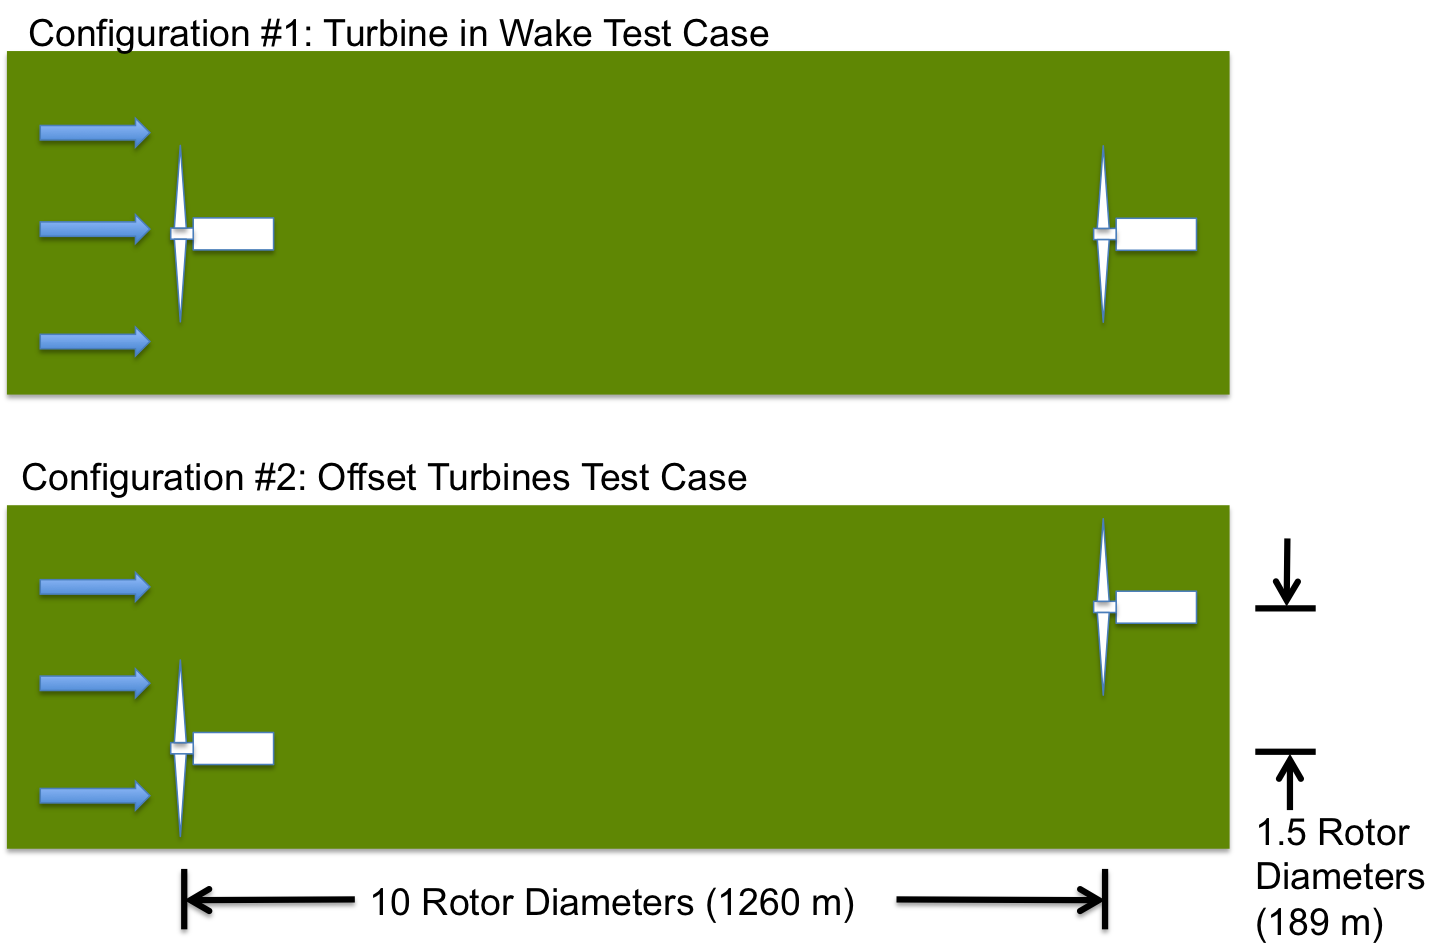
\includegraphics[width = \linewidth]{Figures/ch6Figures/fig6-1.png}
		\rule{35em}{0.5pt}
	\caption{Configurations for SOWFA simulations of feed forward derating control.}
	\label{fig6-1}
\end{figure}

Choosing a grid resolution is a compromise. A fine grid captures flow behavior that coarse grids doesn't capture. However, using a fine grid has a higher computational cost than a coarse grid, requiring more cores and/or more time to run a simulation. One way to balance simulation detail and computational cost is to make the grid resolution finer in the areas you are most interested in (such as near the turbine rotor) and coarser in areas that are of less interest (such as far from the turbine). Another way is to make the grid resolution as fine as it needs to be, but not making it any finer. 

For simulations in Section \ref{section5-4-1} (referencing a chapter 5 section that hasn't been inserted yet) a grid resolution of 1 meter was used near the turbine rotor. This near-rotor grid was not very large, extending only 1 rotor diameter upstream, 6 rotor diameters downstream, and 1.4 rotor diameters radially, which is approximately 0.04\% of the simulation domain volume. However, this near-rotor grid contains approximately 11 million cells, which is about 57\% of the cells in the simulation domain. A 1 m $\times$ 1 m $\times$ 1 m grid large enough to encompass the two turbine systems shown in figure \ref{fig6-1} would have a prohibitively large number of cells and have a prohibitively high computational cost. 

To make the computational cost more manageable a 2 meter near-rotor grid resolution will be used for simulations in this chapter. Though simulation results will be less detailed, we still have high confidence in the accuracy of the results. As Section \ref{section5-4-3} shows, even a near-rotor grid resolution of 4 meters yielded good agreement for power generation, rotor thrust, wake vorticity, and momentum deficit.  

%----------------------------------------------------------------------------------------
%	SECTION 4
%----------------------------------------------------------------------------------------

\section{Tuning and Validation of SOWFA Turbine Model} \label{section6-4}

An actuator line model couples SOWFA's LES based atmosphere model to SOWFA's FAST based turbine dynamics model. To get accurate turbine performance from SOWFA, the actuator line model must be tuned. A series of simulations revealed that an actuator line model with 62 elements per blade and a Gausian projection width of 7.5 meters yields good agreement between SOWFA and FAST simulations. These actuator line parameters comply with the best practices recommended by Churchfield, Lee, and Moriarty \cite{churchfield2012} as well as those recommended by Troldborg \cite{troldborg2009}. It is worth noting that the Gausian projection width chosen here is different than the one chosen for SOWFA simulations in Chapter \ref{Chapter5}. This difference is partially due to the use of a 2 meter near-rotor grid resolution, but it is also caused by a difference in tuning requirements. The SOWFA simulations carried out in Chapter \ref{Chapter5} did not model turbine control, so the actuator line was only tuned to produce good agreement on turbine loads and power generation. The Gausian projection width chosen here produces good agreement on controller behavior as well as loading and power generation.

To illustrate the close agreement between SOWFA and FAST simulations a simple test case from chapter 4 was simulated in SOWFA. In that test case the turbine is subjected to a constant 16 m/s wind. At 100 seconds the turbine is derated by 20\%. At 200 seconds the turbine is returned to full rated operation. Figures \ref{fig6-2} through \ref{fig6-6} show FAST and SOWFA simulation results for this test case. We see in the figures that FAST and SOWFA produce nearly identical results for rotor speed, power, and blade root bending moments. There is also good agreement on blade pitch and tower base bending moment. The blade pitch predicted by SOWFA is typically within 1\% of the blade pitch predicted by FAST, but does briefly exceed 1\% when the turbine is returning to full rated operation. The maximum discrepancy is almost 4\% and occurs at a simulation time of 210 second. SOWFA predicts more high frequency oscillations in tower base bending moment than FAST. However, there is close agreement on the magnitudes of the predicted loads. If we disregard the high frequency components of the SOWFA results the tower base bending loads are typically within 1.5\% of the loads predicted y FAST. However, there are larger differences while the turbine is transitioning from derated operation to full rated operation.  

\begin{figure}[htbp]
	\centering
		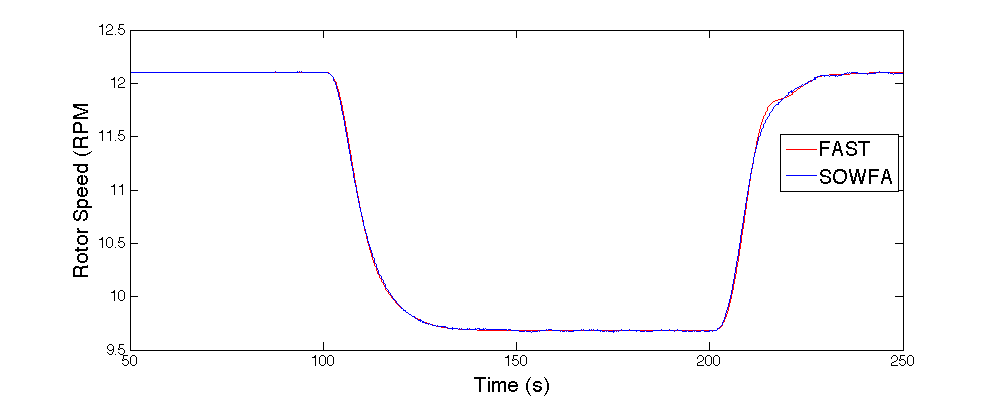
\includegraphics[trim = {1cm 0 2cm 0}, clip, width = \linewidth]{Figures/ch6Figures/fig6-2.png}
		\rule{35em}{0.5pt}
	\caption{Comparison of rotor speed predicted by FAST and SOWFA.}
	\label{fig6-2}
\end{figure}

\begin{figure}[htbp]
	\centering
		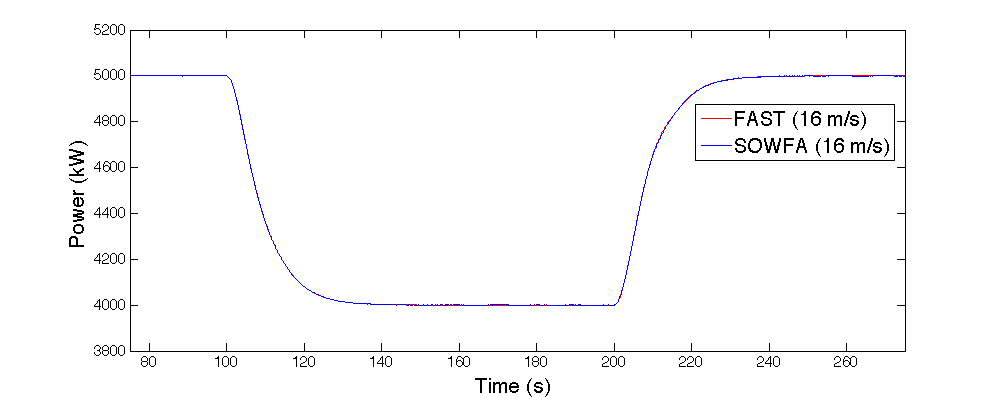
\includegraphics[trim = {1cm 0 2cm 0}, clip, width = \linewidth]{Figures/ch6Figures/fig6-3.png}
		\rule{35em}{0.5pt}
	\caption{Comparison of power predicted by FAST and SOWFA.}
	\label{fig6-3}
\end{figure}

\begin{figure}[htbp]
	\centering
		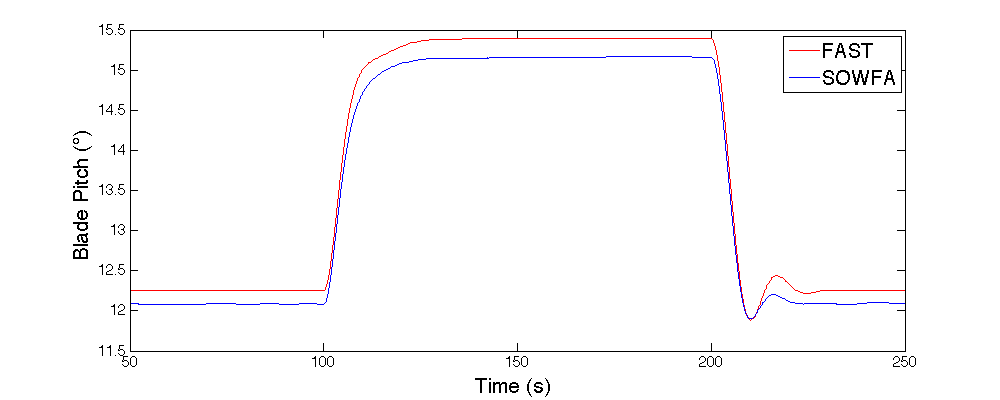
\includegraphics[trim = {1cm 0 2cm 0}, clip, width = \linewidth]{Figures/ch6Figures/fig6-4.png}
		\rule{35em}{0.5pt}
	\caption{Comparison of blade pitch predicted by FAST and SOWFA.}
	\label{fig6-4}
\end{figure}

\begin{figure}[htbp]
	\centering
		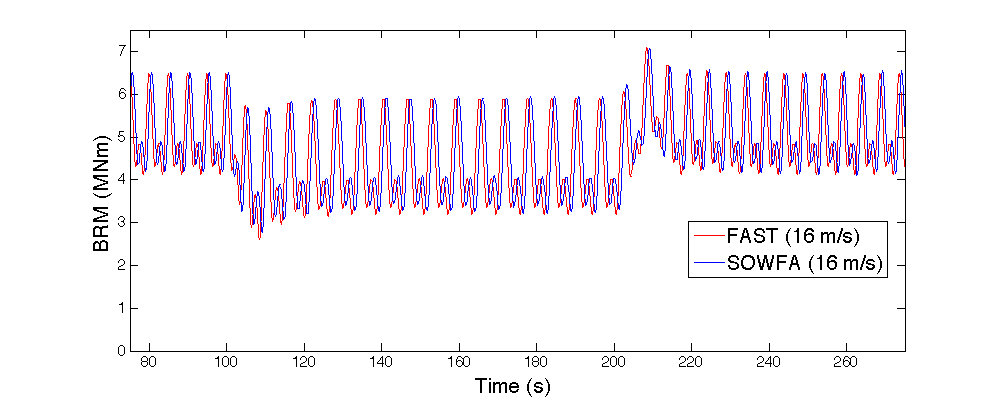
\includegraphics[trim = {1cm 0 2cm 0}, clip, width = \linewidth]{Figures/ch6Figures/fig6-5.png}
		\rule{35em}{0.5pt}
	\caption{Comparison of blade blade root bending moment predicted by FAST and SOWFA.}
	\label{fig6-5}
\end{figure}

\begin{figure}[htbp]
	\centering
		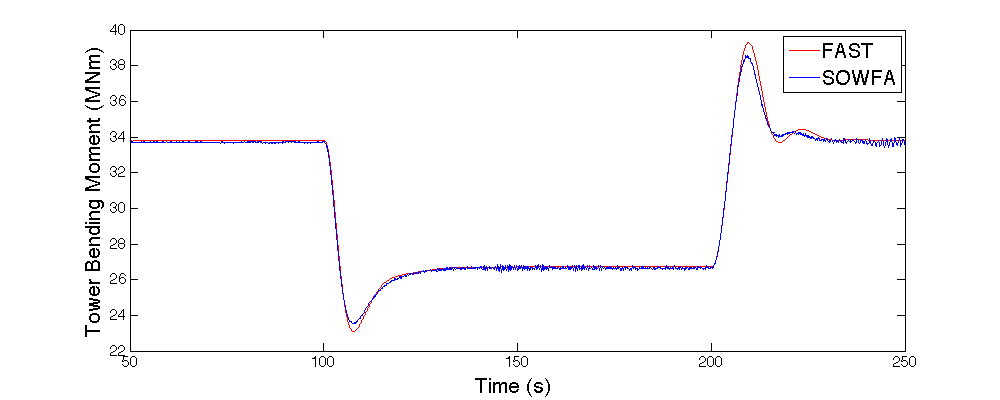
\includegraphics[trim = {1cm 0 2cm 0}, clip, width = \linewidth]{Figures/ch6Figures/fig6-6.png}
		\rule{35em}{0.5pt}
	\caption{Comparison of tower base bending moment predicted by FAST and SOWFA.}
	\label{fig6-6}
\end{figure}

%----------------------------------------------------------------------------------------
%	SECTION 5
%----------------------------------------------------------------------------------------

\section{Gust Modeling in SOWFA} \label{section6-5}

For the FAST simulations in Chapter \ref{Chapter4} gusts are modeled by simply increasing the incoming wind speed. However, this method does not work in SOWFA. SOWFA models airflow as an incompressible fluid in a finite computational domain. Increasing the wind speed across the inlet would cause an increase in the amount of air flowing into the computational domain. Because the fluid is incompressible and constrained, conservation of mass dictates that an increase in the amount of air flowing into the domain be immediately matched by an increase in the amount of air flowing out of the domain and an increase in the amount of air flowing from the input to the output. Therefore, increasing the wind speed across the inlet of the computational domain causes an instantaneous increase in wind speed throughout the computational domain.

To model a gust propagating through a wind farm we must be more subtle. This is done by increasing wind speed across part of the inlet, while decreasing wind speed elsewhere in the inlet. As long as the total amount of air flowing into the domain remains the same, the flow far downstream of the inlet will not be affected. Using this method, the gust is localized near the inlet initially then propagates through the computational domain over time. 

In SOWFA, the user can specify a time varying velocity profile across the inlet by applying a TimeVaryingMappedFixedValue boundary condition. For this boundary condition, the user specifies a list of locations on the inlet plane, then specifying velocities at those points for several simulation times. SOWFA interpolates between the supplied data to determine the velocity profile across the inlet for all time steps in the simulation.

Several inlet velocity profiles were investigated in a series of preliminary SOWFA simulations. The inlet profile was found to have a large effect on how the gust initially appears in the simulation domain and how it behaves as it propagates through the domain. Inlet profiles that confine the gust to a small portion of the inlet were found to give the most control over gust behavior. When the gust covers a large portion of the inlet profile, SOWFA smooths out the effect of the gust. This smoothing effect turns rapid velocity changes at the inlet into more gradual velocity changes within the simulation domain. In the following sections we use inlet profiles that confine the gust to a small portion of the inlet. On the remainder of the inlet, the velocity remains constant. 

In chapter \ref{Chapter4} the turbines were subjected to a hat shaped Extreme Operating Gust as defined in section 6.3.2.2 of IEC61400-1\cite{IEC2005}. Preliminary SOWFA simulations found that it is not possible to simulate a hat shaped gust that will propagate through the SOWFA simulations domain. A hat shaped fluctuation of the inlet velocity begins as a hat shaped gust near the inlet. However, the gust decreased in magnitude and changed shape as it moved through the simulation domain. Instead, simulations in the following sections will model an Extreme Coherent Gust similar to the one defined in section 6.3.2.5 of IEC61400-1. 

Figure \ref{fig6-7} illustrates the difference between an Extreme Operating Gust (EOG) and an Extreme Coherent Gust (ECG). The EOG is a brief fluctuation in wind speed, while the ECG is a sustained increase. IEC1400-1 defines the ECG as a 15 m/s increase in wind speed described by equation \ref{eq6-1}. For simulations in this chapter, the 15 m/s ECG magnitude specified by IEC1400-1 is interpreted to be a maximum coherent gust magnitude, not a required magnitude. If a 15 m/s coherent gust is possible then smaller magnitude coherent gusts are also possible. Coherent gusts were found to propagate through the SOWFA simulation domain with only small changes to the magnitude and shape of the gust, as illustrated in figure \ref{fig6-8}

\begin{figure}[htbp]
	\centering
		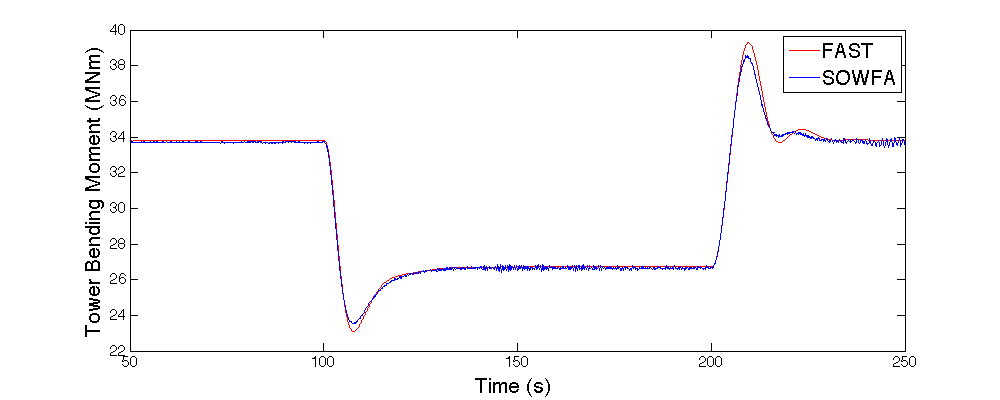
\includegraphics[trim = {1cm 0 2cm 0}, clip, width = \linewidth]{Figures/ch6Figures/fig6-6.png}
		\rule{35em}{0.5pt}
	\caption{Velocity profiles for EOG and ECG.}
	\label{fig6-7}
\end{figure}

\begin{equation}
	U_{gust}=\left\{\begin{matrix}
0 & for  & t<t_{gust}\\ 
 7.5(1-cos(\pi t/10)) m/s & for  & t_{gust} \leq t<(t_{gust}+10)\\ 
 15 m/s &  for & \leq (t_{gust} +10)
\end{matrix}\right. \label{eq6-1}
\end{equation}

\begin{figure}[htbp]
	\centering
		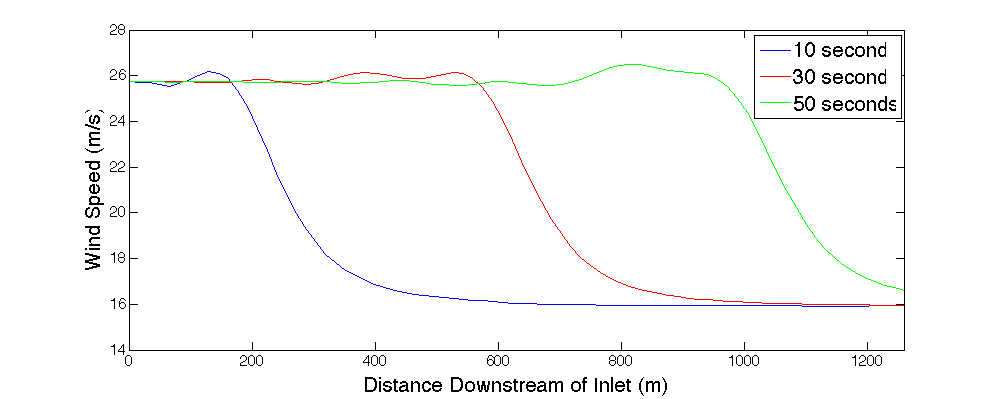
\includegraphics[trim = {1cm 0 2cm 0}, clip, width = \linewidth]{Figures/ch6Figures/fig6-8.png}
		\rule{35em}{0.5pt}
	\caption{Center line velocity as ECG propagates through computational domain.}
	\label{fig6-8}
\end{figure}



%----------------------------------------------------------------------------------------
%	SECTION 6
%----------------------------------------------------------------------------------------

\section{Turbine in Wake Test Case} \label{section6-6}

%----------------------------------------------------------------------------------------
%	SECTION 7
%----------------------------------------------------------------------------------------

\section{Offset Turbines Test Case} \label{section6-7}

%----------------------------------------------------------------------------------------
%	SECTION 8
%----------------------------------------------------------------------------------------

\section{Conclusions} \label{section6-8}

